\documentclass[11pt,a4paper]{article}

\usepackage[provide=*,spanish]{babel}
\usepackage[utf8]{inputenc}
\usepackage[T1]{fontenc}
\usepackage{lmodern}
\usepackage[margin=2.35cm]{geometry}
\usepackage{amsmath}
\usepackage{booktabs}
\usepackage{tabularx}
\usepackage{array}
\usepackage{enumitem}
\usepackage{xcolor}
\usepackage{microtype}
\usepackage{parskip}
\usepackage{titlesec}
\usepackage{hyperref}
\usepackage{xurl}
\usepackage{graphicx}
\usepackage{caption}
\usepackage{float}

\definecolor{azulWCD}{RGB}{17,67,112}
\definecolor{rojoAviso}{RGB}{160,40,30}

\hypersetup{
  colorlinks=true,
  linkcolor=azulWCD,
  urlcolor=azulWCD,
  pdftitle={Respuesta de referencia del WCD al flujo emergente de un suelo seco: seccion 4.6},
  pdfauthor={Jaime A. Betancourt}
}

\titleformat{\section}{\normalfont\Large\bfseries\color{azulWCD}}{\thesection}{0.6em}{}
\titleformat{\subsection}{\normalfont\large\bfseries\color{azulWCD}}{\thesubsection}{0.6em}{}

\newcommand{\ok}{\textcolor{green!50!black}{\textbf{OK}}}
\newcommand{\alerta}{\textcolor{rojoAviso}{\textbf{Revisar}}}
\newcommand{\nota}{\textcolor{orange!80!black}{\textbf{Nota}}}
\newcommand{\archivo}[1]{\path{#1}}

\title{\color{azulWCD}\textbf{Respuesta de referencia del WCD al flujo de neutrones
emergentes de un suelo seco (Bucaramanga)}\\[0.3em]
\large Informe corto de la sección 4.6 de la tesis y base para la calibración CRNS}
\author{Jaime A. Betancourt}
\date{27 de septiembre de 2026}

\begin{document}
\maketitle

\begin{abstract}
Se resume la sección 4.6 de la tesis \emph{Evaluación mediante simulación Monte Carlo de un
detector Cherenkov de agua dopado con NaCl para la medición de neutrones cósmicos con
aplicación en monitoreo de humedad del suelo en Colombia} (páginas impresas 253--263). La
sección continúa la 4.5 (flujo emergente de un suelo seco, revisada en
\archivo{analysis/flujo-bucaramanga_secciones-4.3-4.5/}) y comprende el apartado 4.6.0.1
(construcción de una curva de calibración del WCD) y la subsección 4.6.1 (alcance e
incertidumbres). \textbf{Los únicos datos numéricos existentes son los de la Tabla~4.23}: el
número de neutrones incidentes por intervalo de energía y la eficiencia del WCD en cuatro
medios. Todo lo demás es metodología propuesta. Aquí se reproduce la Tabla~4.23, se derivan de
ella algunas magnitudes adicionales y se señala qué afirmaciones de la sección se apoyan en
esos datos y cuáles quedan como trabajo futuro.
\end{abstract}

\section{Datos disponibles: Tabla 4.23}

La Tabla~4.23 combina el espectro de 207\,969 neutrones ascendentes del suelo seco
(\archivo{filtered_neutrons.shw}, 12~h sobre 1~m$^2$) con las eficiencias monoenergéticas del
WCD, $\varepsilon_j(E_i)$, mediante la suma discreta (Ec.~4.101/4.103 de la tesis)
\begin{equation}
N_{\mathrm{det},j}=\sum_i N_\mathrm{inc}(E_i)\,\varepsilon_j(E_i).
\end{equation}
Los intervalos se construyen con medias geométricas entre energías representativas
(\archivo{Medicion-humedad.ipynb}, celda 2). Como el espectro sólo cubre
10.0011--10\,000.2~meV, los intervalos efectivos son los de la Tabla~\ref{tab:423}.

\begin{table}[H]
\centering\footnotesize\setlength{\tabcolsep}{3.5pt}
\caption{Tabla 4.23 reconstruida. $\varepsilon$ en \%; $N_\mathrm{det}$ redondeado.}
\label{tab:423}
\begin{tabular}{rrr rr rr rr rr}
\toprule
$E_i$ & Intervalo efectivo & $N_\mathrm{inc}$ & \multicolumn{2}{c}{Agua pura} &
\multicolumn{2}{c}{NaCl 2.5 \%} & \multicolumn{2}{c}{NaCl 5 \%} & \multicolumn{2}{c}{NaCl 10 \%}\\
\cmidrule(lr){4-5}\cmidrule(lr){6-7}\cmidrule(lr){8-9}\cmidrule(lr){10-11}
(meV) & (meV) & & $\varepsilon$ & $N_\mathrm{det}$ & $\varepsilon$ & $N_\mathrm{det}$ &
$\varepsilon$ & $N_\mathrm{det}$ & $\varepsilon$ & $N_\mathrm{det}$\\
\midrule
10    & 10.0--15.8    & 12\,485 & 11.829 & 1\,477 & 15.948 & 1\,991 & 18.638 & 2\,327 & 23.417 & 2\,924\\
25    & 15.8--44.7    & 55\,828 & 13.962 & 7\,795 & 18.457 & 10\,304 & 21.563 & 12\,038 & 26.474 & 14\,780\\
80    & 44.7--89.4    & 42\,311 & 15.942 & 6\,745 & 20.761 & 8\,784 & 24.103 & 10\,198 & 29.661 & 12\,550\\
100   & 89.4--173     & 22\,026 & 16.157 & 3\,559 & 21.349 & 4\,702 & 24.710 & 5\,443 & 30.107 & 6\,631\\
300   & 173--387      & 15\,525 & 17.149 & 2\,662 & 22.512 & 3\,495 & 25.922 & 4\,024 & 31.204 & 4\,844\\
500   & 387--592      & 7\,639  & 17.743 & 1\,355 & 22.817 & 1\,743 & 26.628 & 2\,034 & 31.610 & 2\,415\\
700   & 592--837      & 6\,233  & 17.704 & 1\,103 & 22.756 & 1\,418 & 26.377 & 1\,644 & 31.467 & 1\,961\\
1000  & 837--3162     & 24\,280 & 17.984 & 4\,367 & 22.927 & 5\,567 & 26.631 & 6\,466 & 31.753 & 7\,710\\
10000 & 3162--10000   & 21\,642 & 17.871 & 3\,868 & 23.417 & 5\,068 & 26.396 & 5\,713 & 31.653 & 6\,850\\
\midrule
\multicolumn{2}{l}{Total} & 207\,969 & & 32\,931 & & 43\,073 & & 49\,887 & & 60\,665\\
\bottomrule
\end{tabular}
\end{table}

\textbf{Verificación.} Los productos $N_\mathrm{inc}\varepsilon$ y los cuatro totales se
reproducen exactamente (\ok), al igual que $\sum N_\mathrm{inc}=207\,969$ y los incrementos
$\Delta_{2.5\%}=30.8\,\%$, $\Delta_{5\%}=51.5\,\%$ y $\Delta_{10\%}=84.2\,\%$ (Ecs.~4.98--4.100).
Script: \archivo{scripts/verificar_tabla_4_23.py}; salidas en \archivo{resultados/}.

\begin{figure}[H]
\centering
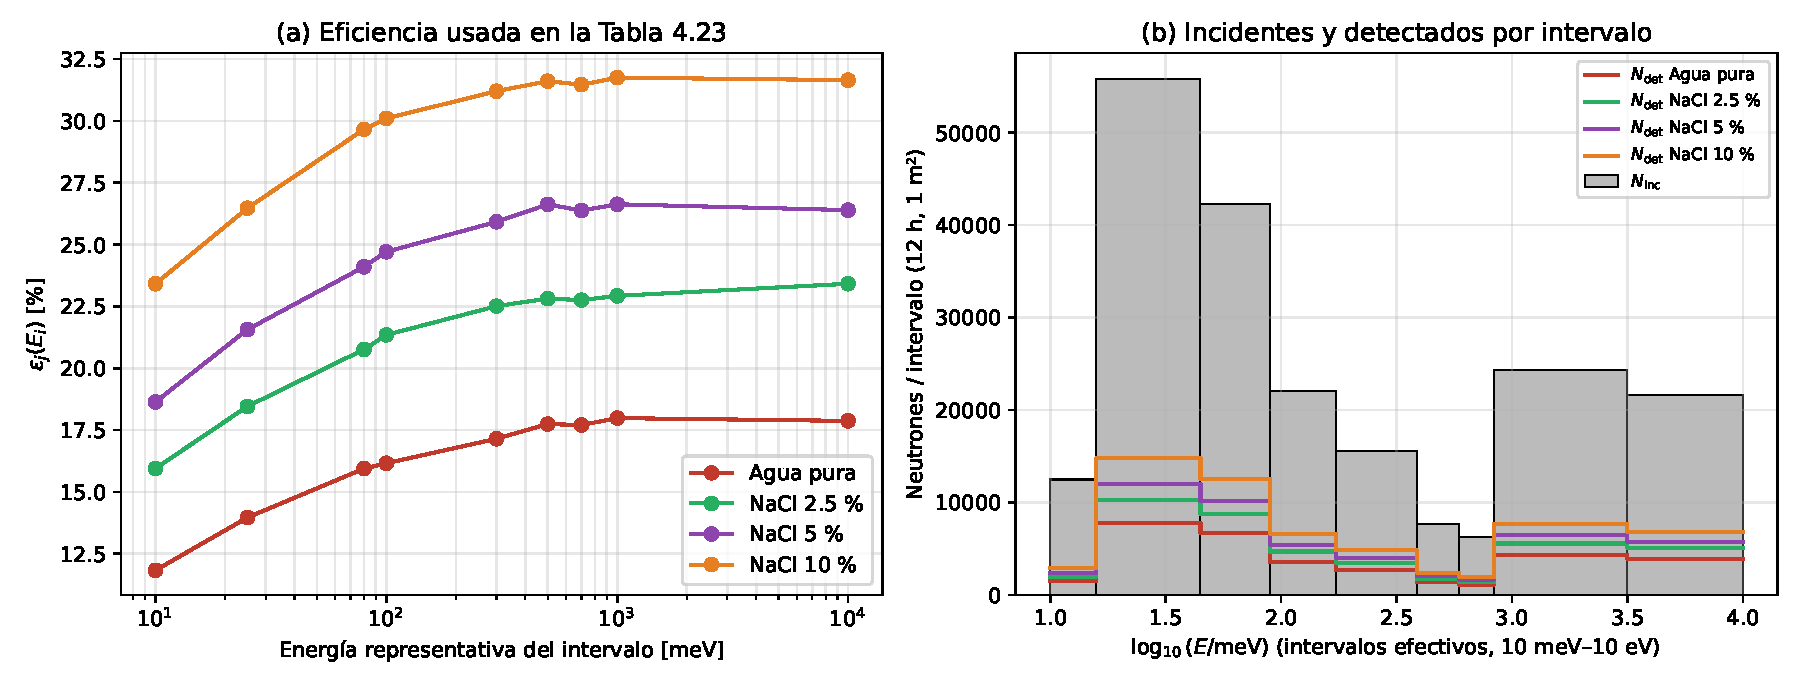
\includegraphics[width=\textwidth]{figuras/tabla_4_23_eficiencia_y_conteos.pdf}
\caption{(a) Eficiencia $\varepsilon_j(E_i)$ usada en la Tabla~4.23. (b) Neutrones incidentes
(gris) y detectados por medio en cada intervalo efectivo del espectro seco.}
\label{fig:eps}
\end{figure}

\subsection*{Magnitudes derivadas sólo de la Tabla 4.23}

\begin{table}[H]
\centering\footnotesize\setlength{\tabcolsep}{4pt}
\begin{tabular}{lrrr>{\raggedleft\arraybackslash}p{2.6cm}r}
\toprule
Medio & $N_{0,j}$ & $\sigma_\text{Poisson}$ & $\bar\varepsilon_j=N_{0,j}/N_\mathrm{inc}$ &
Fracción de $N_{0,j}$ en 10--173~meV & $\varepsilon(10\,\text{eV})/\varepsilon(10\,\text{meV})$\\
\midrule
Agua pura  & 32\,931 & 73  (0.22 \%) & 15.8 \% & 59.4 \% & 1.51\\
NaCl 2.5 \% & 43\,073 & 95  (0.22 \%) & 20.7 \% & 59.9 \% & 1.47\\
NaCl 5 \%   & 49\,887 & 110 (0.22 \%) & 24.0 \% & 60.1 \% & 1.42\\
NaCl 10 \%  & 60\,665 & 134 (0.22 \%) & 29.2 \% & 60.8 \% & 1.35\\
\bottomrule
\end{tabular}
\end{table}

\begin{itemize}[leftmargin=*,itemsep=2pt]
\item El 63.8~\% de los neutrones incidentes cae en los cuatro primeros intervalos
  (10--173~meV, $E_i\le100$~meV), y de allí sale cerca del 60~\% de las cuentas en los cuatro medios.
\item $\sigma_\text{Poisson}=\sqrt{\sum_i\varepsilon_i^2N_{\mathrm{inc},i}}$ incluye sólo la
  fluctuación del espectro. La Tabla~4.23 no da el número de primarios de cada simulación de
  eficiencia, así que la incertidumbre binomial de $\varepsilon$ no se puede propagar. Aun así,
  las diferencias entre medios (miles de cuentas) son mucho mayores que $\sigma$.
\item La eficiencia crece con $E$ hasta $\sim$300--500~meV y luego es casi plana. El cociente
  $\varepsilon(10\,\text{eV})/\varepsilon(10\,\text{meV})$ baja de 1.51 (agua) a 1.35 (10~\%
  NaCl): \emph{el NaCl eleva la eficiencia y además la hace menos dependiente de la energía},
  sobre todo en la región térmica. Por eso la respuesta a un cambio de forma del espectro con la
  humedad será algo distinta en cada medio. Es un argumento a favor de convolucionar con
  $\varepsilon_j(E)$ y no con una eficiencia promedio (Ec.~4.112).
\end{itemize}

\section{Resumen de la sección 4.6}

\paragraph{Introducción de 4.6 (Tabla 4.23).} La mayor población está en 25~meV (55\,828),
seguida por 80~meV (42\,311) y 1000~meV (24\,280) (\ok). El detector con 10~\% de NaCl registra
$1.84\times$ las cuentas del agua pura. La tesis ya reconoce que 10~meV--10~eV cubre sólo la
parte térmica y el inicio de la epitérmica, no toda la banda CRNS (0.1~eV--1~MeV, Köhli y col.,
2018). También reconoce que sólo se calculó la condición seca, de modo que \emph{no se demuestra
sensibilidad a la humedad ni se obtiene una calibración}.

\paragraph{4.6.0.1 Curva de calibración: apartados.}
\begin{description}[leftmargin=0pt,itemsep=3pt,font=\normalfont\bfseries]
\item[Respuesta de referencia (seca).] Define $N_{0,j}\equiv N_{\mathrm{det},j}(\theta_v=0)$ =
  32\,931, 43\,073, 49\,887 y 60\,665 (Ecs.~4.106--4.109). Es el \emph{único resultado numérico}
  del apartado. La tesis aclara correctamente que no es el $N_0$ de un sensor CRNS comercial.
\item[Extensión a varias humedades.] Propone simular
  $\theta_v=0,0.02,\dots,0.40$~m$^3$\,m$^{-3}$ y calcular
  \[N_{\mathrm{det},j}(\theta_v)=AT\!\int\Phi_n(E,\theta_v)\,\varepsilon_j(E)\,dE.\]
  \emph{No simulado.}
\item[Respuesta normalizada.] $R_j(\theta_v)=N_{\mathrm{det},j}(\theta_v)/N_{0,j}$, con
  $R_j(0)=1$, y su inversa $\theta_v=F_j(R_j)$. Definición.
\item[Comparación con la función estándar.] Contrasta con
  $\theta=a_0/(N_\mathrm{corr}/N_0-a_1)-a_2$ y propone ajustar
  $\theta_v=A_j/(R_j-B_j)-C_j$ o $R_j=A_j+B_j e^{-C_j\theta_v}$. Sin datos para ajustar.
\item[Definición experimental de $N_\mathrm{det}$.] Integral del histograma de fotoelectrones
  menos el fondo escalado, $\sum_k[N_k^{s+b}-\alpha_\text{bg}N_k^{b}]$, en una ventana
  $[Q_\text{mín},Q_\text{máx}]$ fija. Definición.
\item[Sensibilidad.] $S_j=-(1/R_j)\,dR_j/d\theta_v$. La tesis dice correctamente que no se
  puede calcular con un único punto seco, y que la mayor tasa con 10~\% NaCl no garantiza
  por sí sola una mejor resolución en $\theta_v$.
\item[Procedimiento experimental.] $R_\text{det}=N_\mathrm{det}/T$, corregida por presión,
  intensidad incidente y vapor de agua; pares $(R_{\text{corr},k},\theta_{v,k})$ con muestreo
  gravimétrico dentro de la huella; $R_0$ ajustable como el $N_0$ convencional. Propuesta.
\item[Esquema general.] $\theta_v\to\Phi_n(E,\theta_v)\to\varepsilon_\text{WCD}(E)\to
  N_\mathrm{det}(\theta_v)\to N_\mathrm{det}/N_0\to\theta_v=F_\text{WCD}$ (Ec.~4.129).
\end{description}

\paragraph{4.6.1 Alcance e incertidumbres.} Sostiene tres conclusiones: el NaCl redistribuye
los destinos hacia la captura (dominada por $^{35}$Cl); ese aumento se propaga a la respuesta
Cherenkov/fotoelectrónica; y la condición seca da una referencia calculada. Declara que las
incertidumbres son sólo estadísticas y enumera los sistemáticos pendientes: biblioteca nuclear,
lista de física, composición y densidad de la solución, índice de refracción, longitudes
ópticas, reflectividad del Tyvek, eficiencia cuántica, geometría, umbral y espectro angular.
Pide propagar la incertidumbre por neutrón primario (lotes o \emph{bootstrap}) y no con
$\sqrt{N}$ de secundarios. Prioridades: $R(E,\theta)$ hasta 1~MeV, varias humedades y
contraste con campo. Concluye que el resultado es una \emph{demostración metodológica y línea
base seca}, no un sensor calibrado. Esta conclusión es coherente con los datos existentes (\ok).

\section{Observaciones para corregir en la tesis}

\begin{enumerate}[leftmargin=*,itemsep=2pt]
\item \alerta\ En ``Respuesta de referencia para la condición seca'' se dice que los
  207\,969 neutrones están ``entre 1~meV y 1~keV''. El espectro cubre \textbf{10~meV--10~eV}.
  Lo que llega hasta 1~keV ($10^6$~meV) es la tabla de eficiencias. Los intervalos de
  100~eV y 1~keV quedan vacíos.
\item \alerta\ Por la misma razón, la frase ``la convolución omite la respuesta entre 1~keV
  y el límite CRNS'' se queda corta: con este espectro no hay neutrones por encima de
  10~eV, así que también falta la banda 10~eV--1~keV.
\item \nota\ Los intervalos son muy desiguales: ``1000~meV'' abarca 837--3162~meV y
  ``10\,000~meV'' abarca 3162--10\,000~meV. Se evalúa $\varepsilon$ en un único punto de cada
  intervalo. Como la eficiencia es casi plana por encima de 500~meV, el efecto es pequeño, pero
  conviene decirlo (la tesis ya pide que $\varepsilon(E_i)$ sea el promedio sobre el intervalo).
\item \nota\ Las $\varepsilon_j$ vienen de haces monoenergéticos a incidencia normal. Los
  neutrones de albedo llegan con una distribución angular amplia. $N_{0,j}$ debe describirse
  como una estimación y no como una simulación directa del espectro en el WCD.
\item \nota\ $\bar\varepsilon$(agua) = 15.8~\% frente a una captura de 23.5~\% (Tabla~4.21)
  para el mismo espectro inyectado. Las dos magnitudes miden cosas distintas: detección con
  criterio fotoelectrónico frente a captura nuclear. Debe declararse el criterio de detección
  que define $\varepsilon$.
\item \nota\ El suelo ``seco'' se describe como una condición sin el hidrógeno del agua, pero
  la composición del suelo usado en la cadena ARTI+suelo no está documentada en las carpetas
  revisadas.
\item \nota\ Formato: ``4.6.0.1'' aparece como \texttt{\textbackslash subsubsection} sin
  subsección padre. Conviene convertirlo en 4.6.1 y renumerar ``Alcance científico'' como
  4.6.2. También conviene citar los coeficientes estándar $a_0=0.0808$, $a_1=0.372$ y
  $a_2=0.115$ de la Ec.~4.118 (Desilets y col., 2010).
\end{enumerate}

\section*{Contenido de la carpeta}
\archivo{informe/} (este documento y su figura), \archivo{resultados/}
(\archivo{tabla_4_23_reconstruida.csv}, \archivo{resumen_respuesta_referencia_seca.csv}) y
\archivo{scripts/verificar_tabla_4_23.py}. El notebook original que genera la Tabla~4.23 es
\archivo{Medicion-humedad.ipynb} (celda 2), ya incluido en
\archivo{analysis/flujo-bucaramanga_secciones-4.3-4.5/notebooks/4.5_suelo-seco/}.

\end{document}
